\documentclass[../CourseManual.tex]{subfiles}

\begin{document}

\subsection{Hegselmann-Krause Dynamics} \label{H-K Dynamics}
The Hegselmann-Krause dynamics are used to simulate opinion changes within systems of agents, with agents moving based on the influence of agents around them. These systems can be used to model influence fields in social media, the spread of fake news, or other situations where agents’ views or positions are altered by the agents around them.

\subsubsection{One-Dimensional Dynamics} \label{One-Dimensional Dynamics}
In the one-dimensional opinion algorithm, each agent has a communication radius of $r_{c_i} \in \mathbb{R}_{>0}$. The position of the agents is stored in $\vec{q}$, a $n \times 1$ matrix, where $n$ is the number of agents. The $i$th agent's position is denoted as $q_i$. The adjacency matrix is an $n \times n$ matrix with each entry determined using
\[
A(i,j) = 
\begin{cases}
1, \text{ if } |q_i - q_j| \leq r_{c_i}, \\
0, \text{ if } |q_i - q_j| > r_{c_i}.
\end{cases}
\]
In situations when $r_{c_i} \neq r_{c_j}$, $A$ will be asymmetric. The degree matrix, $D$, is an $n \times n$ matrix, defined as
\[
D(i,i) = \sum_{j=1}^{n}{A(i,j).}
\]
The Laplacian Matrix is then calculated using $L = D - A$ similar to Formation and Flocking algorithms. Again, the dynamics of $\dot{\vec{q}} = -L\vec{q}$ are used. The discrete version of the position update formula will therefore be
\[
\boldsymbol{q}(t+\Delta t) = \boldsymbol{q}(t) - L \cdot \boldsymbol{q}(t) \cdot \Delta t,
\]
where $\Delta t \in \mathbb{R}_{>0}$ is the user defined time-step between iterations of the simulation. Note: You may recognize these dynamics from the formation algorithm in \hyperref[Formation Consensus Dynamics]{Section \ref{Formation Consensus Dynamics}}. That’s because the opinion algorithm functions in a very similar way, with agents moving to what they perceive as the consensus position based on the other agents within their radius of communication.

\subsubsection{Two-Dimensional Dynamics} \label{Two-Dimensional Dynamics}
The two-dimensional dynamics are very similar to the one-dimensional dynamics. Each agent has a radius of communication $r_{c_i} \in \mathbb{R}_{>0}$ and a position ${q}_i \in \mathbb{R}^2$ with an overall $n \times 2$ position vector, $\boldsymbol{q}$. The adjacency matrix, $A$, is an $n \times n$ matrix defined as:
\[
A(i,j) = 
\begin{cases}
1, \text{ if } ||{q}_i - {q}_j|| \leq r_{c_i}, \\
0, \text{ if } ||{q}_i - {q}_j|| > r_{c_i},
\end{cases}
\]
where $||.||$ is the Euclidean norm. The matrices of $D$ and $L$ are both defined in the same manner as in the one-dimensional case. Following a discrete-time system, the position of each agent is updated using
\[
\boldsymbol{q}(t+\Delta t) = \boldsymbol{q}(t) - L \cdot \boldsymbol{q}(t) \cdot \Delta t.
\]
The two-dimensional dynamics simulate networks with more complicated opinion profiles, with agents being swayed in two different directions independently. For instance, a two-dimensional opinion could be a model of political inclinations, where agents fall on both an economic spectrum
and a social spectrum, which could be treated independently of each other.

\subsection{Simulation App} \label{Simulation App: Opinion}
The app provided uses the consensus dynamics defined in \hyperref[H-K Dynamics]{Section \ref{H-K Dynamics}} to update each agent’s location for every iteration of the simulation. The critical components of the apps functionality have been inserted into external functions, which you will be required to create in order to get the app functioning.  The functions that you will be responsible for are discussed in detail in \hyperref[MATLAB Functions: Opinion]{Section \ref{MATLAB Functions: Opinion}}.  Upon simulation completion, the  app  will  create  an  excel  file  containing  the  position  of  each  agent  for  every  iteration  of  the simulation.  This data can then be used to conduct further analysis on the results to improve or validate your design.

%app picture goes before the descriptions
\begin{figure}[H]
    \centering
    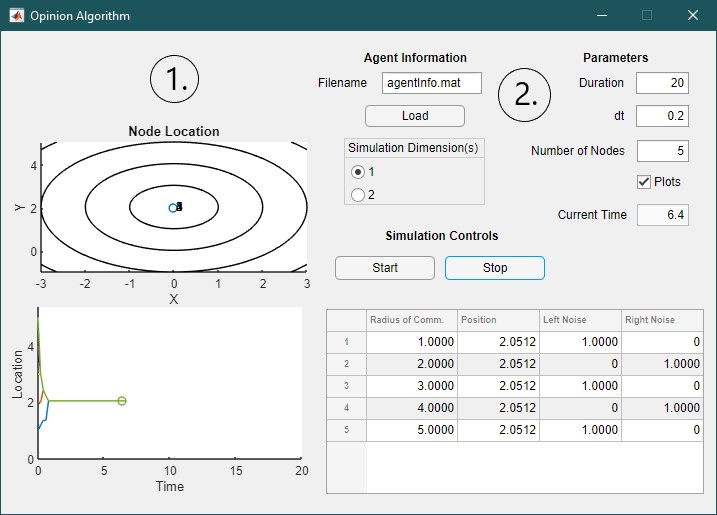
\includegraphics[width=350pt]{media/Opinion.jpg}
    \caption{Screen capture of OpinionApp.mlapp with default settings}
    \label{fig: opinion app}
\end{figure}

\subsubsection{Plots} \label{Plots: Opinion}
Area 1 of Figure \ref{fig: opinion app} displays the plots section of the the Opinion app. This section contains two separate plots: the \textbf{Node Location} plot and the \textbf{Node Trajectory} plot. \\

Note: With one-dimensional dynamics, both plots are displayed; however, for the two-dimensional dynamics, the \textbf{Node Trajectory} plot is removed. \\

The \textbf{Node Location} plot displays the current location of each agent in the form of a circular marker. In addition, for each agent, a thin black circle with a radius matching the radius of communication of the agent is displayed to visualise the communication range on the agent. \\ 
The \textbf{Node Trajectory} plot displays each agent's position as the simulation progresses. \\

\subsubsection{User Controls} \label{User Controls: Opinion}
Area 2 of Figure \ref{fig: opinion app} displays the user controls section of the Opinion app. This section is divided into 3 sub-sections: the \textbf{Agent Information} sub-section, the \textbf{Parameters} sub-section, and the \textbf{Simulation Controls} sub-section. \\

In the \textbf{Simulation Controls} sub-section, the \textbf{Start} button starts the simulation and the \textbf{Stop} button stops the simulation. \\

Simulation parameters can be modified in the \textbf{Parameters} sub-section. The number of nodes in the simulation can be updated using \textbf{Number of Nodes} field. The \textbf{dt} field is used to adjust the simulation time step, $\Delta t$. The length of time that the simulation runs for can be modified in the \textbf{Duration} field. The \textbf{Current Time} field displays the current simulation time. The \textbf{Plots} checkbox, when enabled, will update the \textbf{Node Location} plot, the \textbf{Node Trajectory} plot (if applicable), and the \textbf{Node Information} table on every iteration. Disabling \textbf{Plots} will greatly increase the speed of your simulation. This is useful if you need to simulate for more than a few hundred iterations. \\

When running a one-dimensional simulation, the data entry table will contain four columns with the headings of \textit{Radius of Communication} \textit{Position}, \textit{Left Noise}, and \textit{Right Noise}. Switching to the two-dimensional simulation will have the data entry table reconfigured with the headings of \textit{Radius of Communication}, \textit{X Position}, and \textit{Y Position}. This table can be filled in manually each time the app is opened, or loaded into the app using a .mat file under the \textbf{Agent Information} section. Using the .mat loading feature will save you time by not having to write in the agent data each time the app is opened.

\subsubsection{Matrix Editor} \label{Matrix Editor: Opinion}

The \textbf{Matrix Editor Opinion} app allows for the user to save the initial conditions for the nodes in the simulation for either simulation dimension setting. For either dimension setting, the columns in the table are similar to those that would be shown in the Opinion App. The number of rows in the table is reflective of the number of nodes you want to have in your simulation. These initial settings can be saved under a user specified .mat file name and also reloaded into the app to be edited at a later point. 

\begin{figure}[H]
    \centering
    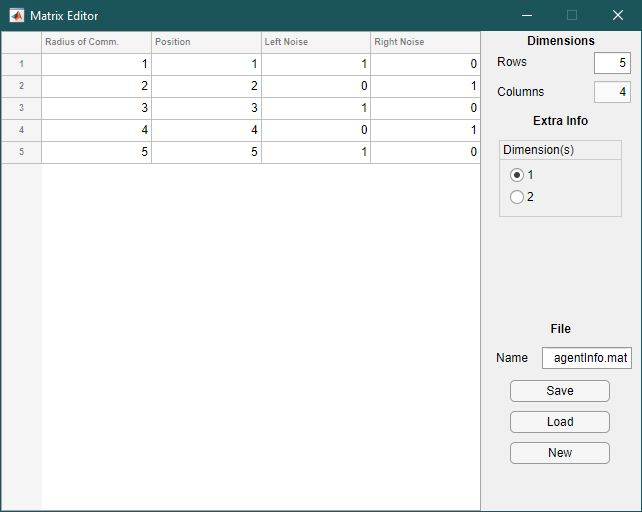
\includegraphics[width=350pt]{media/MatrixEditorOpinion.JPG}
    \caption{Screen capture of MatrixEditorOpinion.mlapp with default settings}
    \label{fig: matrix editor opinion}
\end{figure}

\subsubsection{Parameters and Variables}
\renewcommand{\labelenumi}{\roman{enumi}}
\begin{enumerate}

    \item Number of Nodes $(numNodes)$: Total number of nodes $(N)$ used in simulation.
    
    \item Node Data $(nodeData)$: Matrix whose rows store the radius of communication, coordinates, and left and right noise for each agent. 
    
    \item Radius of Communication $(rComm)$: The radius of communication $r^{i}_c$ for node $i$. This value can be constant for all nodes or take different values for each.  
  
    \item Node Position $(nodePosition)$: An $N \times dim$ matrix where row $i$ describes the positional information of the $i^{th}$-node. For example, in the 1-D and 2-D cases respectively we have: 
    
    $$nodePosition\_1D = 
    \begin{bmatrix}
    q^{1}\\
    q^{2}\\
    \vdots\\
    q^{N}\\
    \end{bmatrix}, \qquad
    nodePosition\_2D = 
    \begin{bmatrix}
    q^{1}_{x} \hspace{0.5cm} q^{1}_{y}\\
    q^{2}_{x} \hspace{0.5cm} q^{2}_{y}\\
    \vdots \hspace{0.5cm} \vdots \\
    q^{N}_{x} \hspace{0.5cm} q^{N}_{y}\\
    \end{bmatrix}$$
    
    \item Left Noise $(leftNoise)$: Random noise taking values between 0 and 1 (inclusive) applied to the positional information of the agent.  This parameter is only present in the 1-D simulation case. 
    
    \item Right Noise $(rightNoise)$: Random noise taking values between 0 and 1 (inclusive) applied to the positional information of the agent.  This parameter is only present in the 1-D simulation case. 
    
    \item Adjacency Matrix $(A)$: The $N \times N$ adjacency matrix.  $A$ must not necessarily be symmetric. 
  
    \item Degree Matrix $(D)$: The $N \times N$ degree matrix:
    
    \[
    D(i,i) = \sum_{j=1}^{n}{A(i,j)}.
    \]
    
    
    \item Laplacian Matrix $(L)$: The $N \times N$ Laplacian matrix:
    
    $$L = D - A$$

    \item Duration $(duration)$: Total duration the simulation will run for.
    
    \item $\Delta t$ $(dt)$: Amount of time simulated in each iteration.
    
    
\end{enumerate}

\subsubsection{MATLAB Functions} \label{MATLAB Functions: Opinion}
You will need to create the following MATLAB functions in order for the simulation to function. The order that functions are listed is the order that you will be creating them during the project.\\

\textbf{calcA.m} -- calcA.m is used to calculate the adjacency matrix. The calcA function takes as input $nodeData$ and outputs $A$. If the simulation is one-dimensional, $A$ is calculated as seen in \hyperref[One-Dimensional Dynamics]{Section \ref{One-Dimensional Dynamics}} with the equation 

$$
A(i,j) = 
\begin{cases}
1, \text{ if } |q_i - q_j| \leq r_{c_i}, \\
0, \text{ if } |q_i - q_j| > r_{c_i}.
\end{cases}
$$

If the simulation is two-dimensional, $A$ is calculated as seen in \hyperref[Two-Dimensional Dynamics]{Section \ref{Two-Dimensional Dynamics}} with the equation 

$$
A(i,j) = 
\begin{cases}
1, \text{ if } ||{q}_i - {q}_j|| \leq r_{c_i}, \\
0, \text{ if } ||{q}_i - {q}_j|| > r_{c_i},
\end{cases}
$$

\textbf{calcL.m} -- calcL.m is used to calculate the Laplacian matrix. The calcL function takes as input $A$ and outputs $L$. $L$ is calculated as seen in \hyperref[One-Dimensional Dynamics]{Section \ref{One-Dimensional Dynamics}} with the equation 

$$L = D - A$$

\textbf{updateNodeData.m} -- updateNodeData.m is used to update the $nodeData$ matrix. This function must update the position of each agent, but it can also update the other node parameters depending on the cost function(s) or condition(s) introduced in the function. The updateNodeData function takes inputs $nodeData$, $L$, $dt$, and $time$, and outputs $nodeData$. If the simulation is one- or two-dimensional, positional data in $nodeData$ is updated as seen in \hyperref[One-Dimensional Dynamics]{Section \ref{One-Dimensional Dynamics}} or \hyperref[Two-Dimensional Dynamics]{Section \ref{Two-Dimensional Dynamics}} with the equation

$$
\boldsymbol{q}(t+\Delta t) = \boldsymbol{q}(t) - L \cdot \boldsymbol{q}(t) \cdot \Delta t,
$$

\subsection{Example: Opinion} \label{Example: Opinion}
This section provides a sample P2 project using the Hegselmann-Krause opinion dynamics algorithm. This example is broken down into what is to be completed each week of the project to provide a reference as to what will be expected with your project. You can not use this application area for your project.

\subsubsection{Week 1} \label{Week 1: Opinion}
\textbf{Area of Application}\\
The application area that has been selected is the spread of fake news within online communities and its influence on political opinions. One of the defining characteristics of the system is trustworthiness, where agents ``trust" the agents closer to them more than those farther away. This represents how individuals are more likely to be swayed by agents that are closer to them, reflecting how individuals are more likely to be swayed by sources they are familiar with and echo their own political views. A method to model this situation amongst a populous of potential voters is desired by a government agency.\\

\textbf{Algorithm Selection}\\
With the area of application decided, the most applicable deployment algorithm from the list of four options must be selected. Based on the system that is to be modelled, the most suitable algorithm to use is the Hegselmann-Krause opinion dynamics.\\

\textbf{Pitch Presentation}\\
With the area of application selected, a brief pitch presentation of the application area was created. This presentation provided a high-level overview of the area of application and how the opinion algorithm could be implemented to generate the appropriate model for the system.

\subsubsection{Week 2} \label{Week 2: Opinion}
\textbf{Proposal Report}\\
With the area of application selected and opinion algorithm selected, the proposal report could then be written. This report provided a background description of the application area, a problem definition and how the deployment algorithm will be applied. The main stakeholders for the project were identified and included; the citizens of a country, social media and news platforms, a government agency and more. Some preliminary design metrics were also included in the report, which included the design parameters that can be varied for the project. Additional research was conducted to determine these various parameters and their applicable range of values.\\

\textbf{Adjacency Matrix}\\
By the standard Hegselmann-Krause dynamics, agents move to the consensus position of all agents within their radius of communication, $r_c$, equally weighing every opinion they can see. For this application, these dynamics do not suit our system since agents are to favour opinions that are closer to their own. To change this, the adjacency matrix can be redefined as:
\[
A(i,j) = 
\begin{cases}
\frac{1}{(1+d)^2}, & \text{if } d \leq r_{c_i},\\
0, & \text{if } d > r_{c_i},
\end{cases}
\]

Where $d = |q_i - q_j|$ in the one dimensional case, and $d = ||\vec{q}_i - \vec{q}_j||$ in the two dimensional case. The communication distance $r_{c_i}$ is a value that would be determined through research. Whether the system is to be 1-dimensional or 2-dimensional will be dependent on the research conducted to determine if there is only one set of influence parameters or if there are two sets of independent influence parameters. An ``influence leader” $k$ could also be introduced by setting:
\[
A(i,k) = 10 \times A(i,k), \forall i \in [1,n],
\]
which will increase the influence that the $k$th agent will have on all other agents by an order of magnitude.

\subsubsection{Week 3} \label{Week 3: Opinion}
\textbf{MATLAB Coding}\\
Using the adjacency matrix determined from Week 2, the code to generate the corresponding adjacency matrix in the simulation can be written in the \textit{calcA.m} function. In addition, the \textit{calcL.m} function can be written by translating the Laplacian matrix equation into MATLAB code.\\

\textbf{Design Process}\\
Continued establishing design metrics to be used to evaluate aspects of the final design solution. An example of one design metric is how quickly focused clusters begin to form. \\

Researched whether the simulation should be 1 dimensional or 2 dimensional. This should be finalized by the beginning of Week 4. Began researching the various components of the Triple Bottom Line (TBL) analysis for the project; social, economic and environmental considerations. This research could include; budget limits of research groups for design solution, performance and more. Determining how these factors will influence the design choices you make is important to keep in mind.\\

\textbf{Reports}\\
Submitted a one page Progress Report that highlighted the team's current position with the project, any challenges faced by the team and strategies to overcome these challenges and complete upcoming tasks.

\subsubsection{Week 4} \label{Week 4: Opinion}
\textbf{MATLAB Coding}\\
With the adjacency and Laplacian matrices calculated, and the dimension of the simulation finalized, the \textit{updateNodeData.m} function that updates the position and other corresponding data parameters (if applicable) for each node in the simulation can be written. The velocity of the nodes can be capped by normalizing the velocity, $\dot{q}_i$, if it exceeds some maximum speed, as can be seen in \hyperref[Example: Formation]{Section \ref{Example: Formation}}.\\ 

\textbf{Design Process}\\
Established methods to evaluate design alternatives. This could include creating an evaluation matrix. If using an evaluation matrix, be sure to justify the categories made and the weights assigned to each category (may require additional research). Certain movements by the nodes may be costly to the node, and thus can be accounted for by introducing a cost function to \textit{updateNodeData.m}. This cost function will require some research and can be fully introduced in Week 5. \\

By the end of Week 4, the simulation should be operational, with most bugs in the code having been resolved.  

\subsubsection{Week 5} \label{Week 5: Opinion}
\textbf{MATLAB Coding}\\
Based on the results from research, an appropriate cost function was introduced to \textit{updateNodeData.m}.\\

\textbf{Design Process}\\
Using the completed simulation, the design parameters of the system can be varied over their appropriate ranges and evaluated against the established design metrics to determine the most optimum design solution. \\

\textbf{Reports}\\
Similar to the first progress report, the second progress report is a one-page summary that highlights the items the team has completed, the challenges the team faces and how they will overcome these challenges.\\

Began work on the final report, which includes the Design Process, Design Solution and its justification, TBL analysis and more. This report should include the updated sections from the proposal report based on the feedback returned.

\subsubsection{Week 6} \label{Week 6: Opinion}
\textbf{Final Design}\\
Complete any remaining testing and design finalization. Generate supporting materials for the final report and final presentation. Completed the final report and presentation.



%Consider a situation where we’re modeling the spread of fake news within online communities. One of the defining characteristics of this system could be trustworthiness, where agents “trust” agents that are closer to them more than agents that are far away. This represents how individuals are likely to be swayed by sources they’re familiar with and that echo their own political views. We know that the standard Hegselmann-Krause dynamics make agents move to the consensus position of all agents within their radius $r_c$, equally weighting every opinion they can see. These dynamics don’t suit our system, as we want agents to favour opinions that are closer to their own. To change this we can redefine the A matrix as:
%\[
%A(i,j) = 
%\begin{cases}
%\frac{1}{(1+d)^2} & \text{if } d \leq r_{c_i}\\
%0 & \text{if } d > r_{c_i}
%\end{cases}
%\]

%Where $d = |q_i - q_j|$ in the one dimensional case, and $d = ||\vec{q}_i - \vec{q}_j||$ in the two dimensional case. The communication distance $r_{c_i}$ is a value that would be determined through research.\\

%This new definition checks if agents can communicate, and then weights the influence of opinion based on the distance between the agents, with smaller distances resulting in greater influence. In this way, it achieves our desired goal. We could also model an ``influence leader” $k$ by setting:
%\[
%A(i,k) = 10 \times A(i,k), \forall i \in [1,N]
%\]
%which increases the influence of the $k$th agent on all other agents by an order of magnitude. Lastly we could cap velocity normalizing $\dot{\vec{q}}_i$ if it exceeds some maximum speed, as seen in \hyperref[Example: Formation]{Section \ref{Example: Formation}}.Please note that all values used in this simulation are fabricated for the purposes of the example. \\

%For your own application, research how agents within your system act. Once you have an understanding of the basic characteristics of the system, you can start altering the algorithm in many ways to simulate your project. Perhaps you want to introduce boundaries that agents can’t cross or define a relationship between the number of agents in contact and the size of $r_c$. There are many possibilities, so be creative when working on your project!

\end{document}